\section{Quantitative account}
\label{sec:quant}

\begin{figure*}[t]
  \centering
  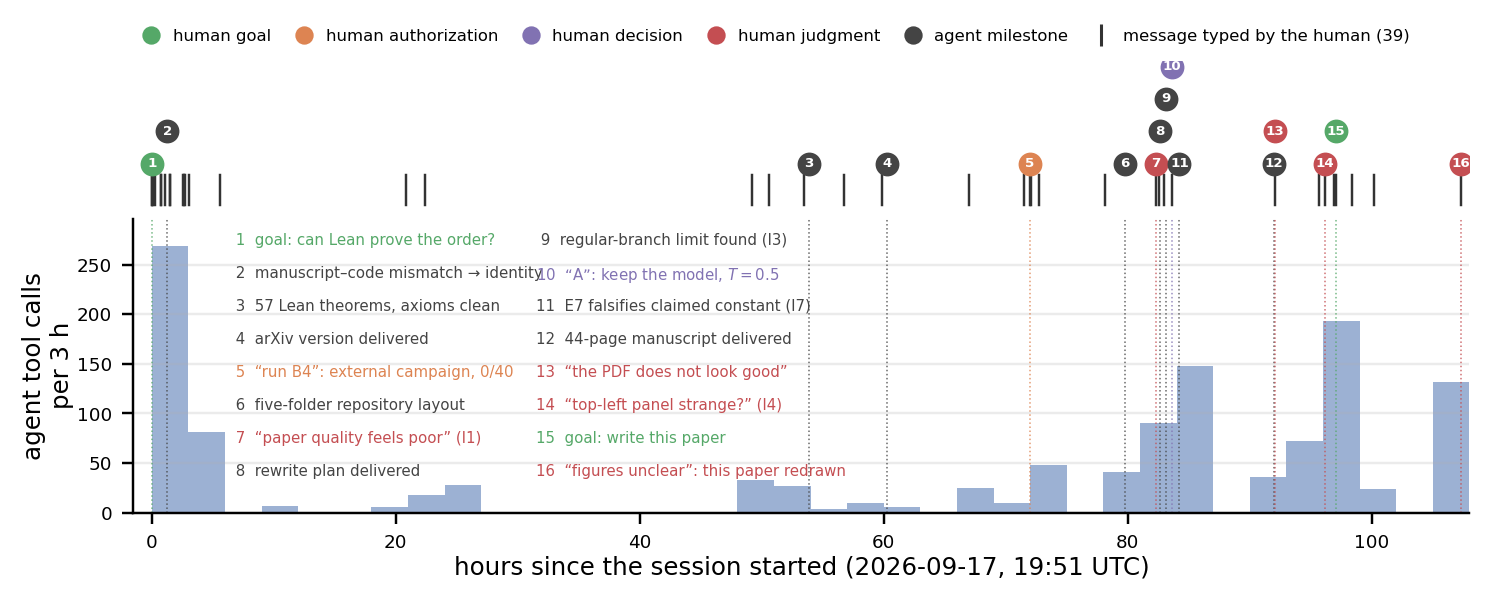
\includegraphics[width=\textwidth]{figures/fig_session.png}
  \caption{The final session, from its transcript. Bars: agent tool calls per three hours. Ticks in
  the strip: the \nHuman{} messages typed by the human. Numbered markers: milestones and the
  human's interventions, keyed in the empty region of the plot and coloured by kind. The identity
  was found within the first two hours (event~2); the rewrite (events 7--12) took about ten hours
  of agent time and four human messages; the two remaining human judgments (13, 14) and the
  request for this paper (15) came after the manuscript was delivered. The gaps are hours in which
  the human was away and the agent idle.}
  \label{fig:session}
\end{figure*}

\paragraph{Effort}
The program left 49 versioned experiments with 793 result files, 341 ledger scripts, 57 Lean
theorems, a 44-page manuscript and 11 memory files (Table~\ref{tab:artefacts},
Appendix~\ref{app:cost}). Figure~\ref{fig:session} profiles the final session, in which the Lean
development was built, the manuscript rewritten and this paper drafted: of its \nTools{} tool
calls about a third were validators and manuscript builds, a third inspection and editing of
files, a tenth Lean, and a twentieth experiments. Earlier phases were not recorded as transcripts
and are documented by the version ledger and the dated logs.

\paragraph{What the human said}
Of the transcript's \nEntries{} user-role entries, \nHarness{} are harness-generated and
\nShell{} are shell commands; \nHuman{} were typed by the human. They fall into six kinds (Appendix~\ref{app:messages}): goals (twelve), approvals of the agent's own proposals
(nine), authorizations (three), decisions (two), judgments (four) and questions (six); the rest
were acknowledgments. None contained a technical instruction about the method, the proofs or the
experiments. The judgments produced Incidents 1 and 4, the layout overhaul of the manuscript and
the redrawing of this paper's figures; the benchmark-horizon decision went against the agent's
recommendation.

\paragraph{What the agent did without being asked}
It chose the experiment set and its reference policy, found and fixed the orientation-angle
formula, discovered and escalated the regular-branch limit, added the alignment check for the
public comparison, wrote the experiment that falsified its own claim, froze the old ledger, and
wrote the memory files for the next session. It also produced the human-caught errors.
